\documentclass[12pt]{article}
\usepackage{graphicx}
\usepackage{amsmath}
\usepackage{float}

\title{Lab 2: Measuring Laser Beam Intensity Profiles}
\author{Arnav Menon \\ School of Physics, Georgia Institute of Technology}
\date{January 29, 2025}

\begin{document}

\maketitle

\section*{Purpose}
This experiment measures the intensity profile of a laser beam, focusing on its spatial distribution. Techniques like the scanning slit and razor blade methods are used to characterize the Gaussian intensity profile, essential for applications in optical communications, laser machining, and medical systems.

\section{Visual Estimate of Beam Width}

\subsection{Theory and Motivation}
The visual estimate method provides a quick approximation of the beam width by observing the beam on a grid pattern. For a Gaussian beam, the intensity profile is:
\[
I(r) = I_0 \exp\left(-\frac{2r^2}{w^2}\right),
\]
where \( I_0 \) is the peak intensity, \( r \) is the radial distance, and \( w \) is the beam width. At \( r = w \), the intensity drops to \( 1/e^2 \) of its peak value.

\subsection{Procedure}
\begin{enumerate}
    \item A 1 mm grid pattern was placed in the beam path.
    \item The beam diameter was visually estimated and divided by 2 to obtain \( w \).
    \item The process was repeated with an O.D. 2 neutral density filter.
\end{enumerate}

\subsection{Analysis and Discussion}
The results, summarized in Table \ref{tab:visual_estimate}, show the beam width remained consistent with and without the filter, confirming that beam width is independent of power. However, the visual estimate is limited by subjective judgment and grid resolution.

\begin{table}[h!]
    \centering
    \begin{tabular}{|c|c|}
        \hline
        \textbf{Parameters with Units} & \textbf{Value} \\
        \hline
        Base Laser Power (V) & 2.83 \\
        Visual Estimate Full Power ($\mu$m) & 500 \\
        Visual Estimate OD 2 ($\mu$m) & 125 \\
        Slit Max Laser Power (V) & 0.704 \\
        Width Estimate from Slit Max ($\mu$m) & 320.741 \\
        Blocked Beam Power (V) & 0.009 \\
        \hline
    \end{tabular}
    \caption{Summary of visual estimate and related measurements.}
    \label{tab:visual_estimate}
\end{table}

\subsection{Conclusion}
The visual estimate provided a quick but less precise approximation of the beam width. It confirmed that beam width is independent of power, but more accurate methods are needed for precise measurements.

\section{Scanning Slit Method}

\subsection{Theory and Motivation}
The scanning slit method measures the intensity profile by translating a narrow slit across the beam. The transmitted power follows a Gaussian distribution:
\[
P(x) \approx \sqrt{\frac{\pi}{2}} I_0 w d \exp\left(-\frac{2(x - x_0)^2}{w_x^2}\right),
\]
where \( d \) is the slit width. Fitting the data to a Gaussian function yields the beam width \( w_x \).

\subsection{Procedure}
\begin{enumerate}
    \item A 100 \(\mu m\) slit was scanned across the beam in 0.005-inch increments.
    \item The transmitted power was measured and converted to milliwatts.
    \item The data was fitted to a Gaussian function.
\end{enumerate}

\subsection{Analysis and Discussion}
The data was fitted to a Gaussian function, as shown in Figure \ref{fig:gaussian_fit}. The fit parameters are summarized in Table \ref{tab:fit_parameters}.

\begin{figure}[h!]
    \centering
    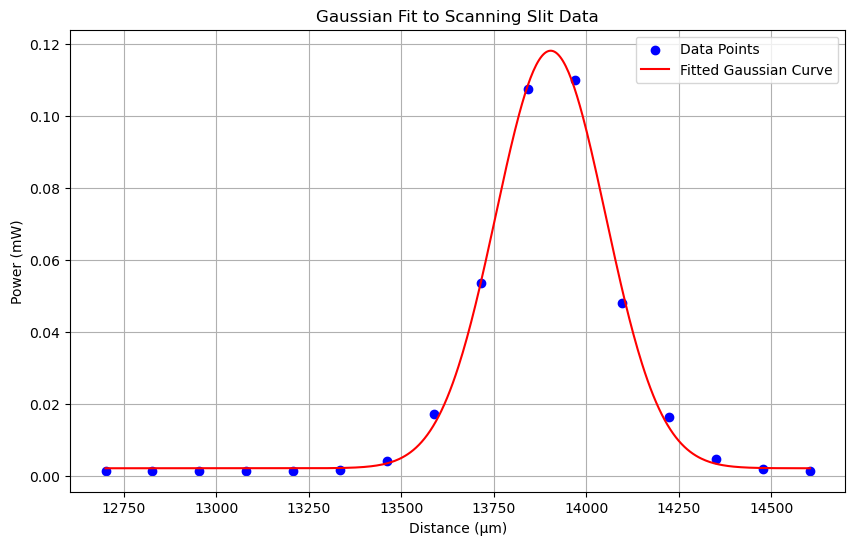
\includegraphics[width=0.8\textwidth]{output.png}
    \caption{Gaussian fit to the intensity profile measured using the scanning slit method.}
    \label{fig:gaussian_fit}
\end{figure}

\begin{table}[h!]
    \centering
    \begin{tabular}{|c|c|}
        \hline
        \textbf{Parameter} & \textbf{Value} \\
        \hline
        \( y_0 \) (background) & 0.002189 mW \\
        \( A \) (amplitude) & 0.116039 mW \\
        \( \text{width} \) (\( w_x \)) & 148.41 \(\mu m\) \\
        \( x_0 \) (center position) & 13903.68 \(\mu m\) \\
        \hline
    \end{tabular}
    \caption{Fit parameters for the Gaussian function.}
    \label{tab:fit_parameters}
\end{table}

The Gaussian fit confirmed the beam's Gaussian intensity profile, with a beam width of 148.41 \(\mu m\). The small background noise and strong signal amplitude indicate reliable measurements.

\subsection{Conclusion}
The scanning slit method provided precise measurements of the beam width and intensity profile, confirming the Gaussian nature of the beam. This method is ideal for beams larger than the slit width.

\section{Scanning Razor Blade Method}

\subsection{Theory and Motivation}
The scanning razor blade method measures the beam width by blocking the beam with a razor blade. The transmitted power follows a complementary error function (erfc):
\[
P(x) = \frac{P_{\text{total}}}{2} \text{erfc}\left(\frac{\sqrt{2}(x - x_0)}{w_x}\right).
\]
Fitting the data to the erfc function yields the beam width \( w_x \).

\subsection{Procedure}
\begin{enumerate}
    \item A razor blade was scanned across the beam in 0.005-inch increments.
    \item The transmitted power was measured and converted to milliwatts.
    \item The data was fitted to an erfc function.
\end{enumerate}

\subsection{Analysis and Discussion}
The data was fitted to an erfc function, as shown in Figure \ref{fig:erfc_fit}. The fitted parameters are:
\begin{itemize}
    \item Amplitude (\( A \)): 0.255794 mW
    \item Center position (\( \mu \)): 13383.28 \(\mu m\)
    \item Beam width (\( \sigma \)): 143.29 \(\mu m\)
    \item Background offset (\( y_0 \)): 0.002827 mW
\end{itemize}

\begin{figure}[h!]
    \centering
    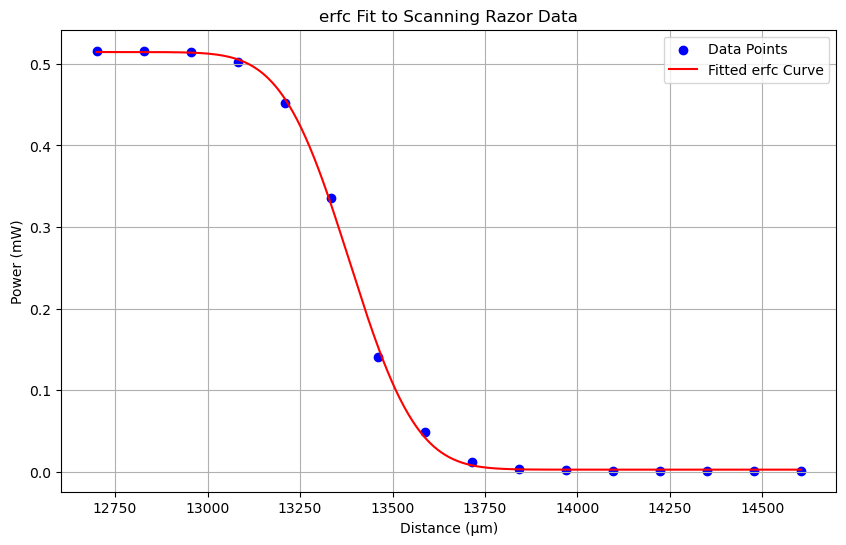
\includegraphics[width=0.8\textwidth]{output2.png}
    \caption{erfc fit to the intensity profile measured using the scanning razor blade method.}
    \label{fig:erfc_fit}
\end{figure}

The erfc fit confirmed the Gaussian intensity profile, with a beam width of 143.29 \(\mu m\), consistent with the scanning slit method.

\subsection{Conclusion}
The scanning razor blade method is effective for measuring small beams, complementing the scanning slit method. The erfc fit provided accurate beam width and center position measurements.

\section{Summary}
Three methods—visual estimate, scanning slit, and scanning razor blade—were used to measure the laser beam's intensity profile. The visual estimate provided a quick approximation but lacked precision. The scanning slit and razor blade methods yielded accurate measurements, confirming the Gaussian intensity profile. These techniques are essential for applications requiring precise beam characterization, such as laser alignment and beam shaping.

\end{document}

